\section*{Linealidades comunes}
En los sistemas físicos se presentan varios tipos de no linealidades; incluirlas permite hacer mejores representaciones matemáticas que se ajusten a la realidad. La literatura ha descrito múltiples modelos de estos fenómenos no lineales \cite{khalil2}\cite{jean}\cite{gene}\cite{ogata}.

En el caso del SLM del dispositivo ECP 730, analizaremos el fenómeno de atascamiento-deslizamiento debido al contacto físico de las superficies entre la varilla de vidrio y el disco. Se considera que el mencionado fenómeno, a su vez, está compuesto por la fricción y la zona muerta.

\begin{figure}
    \begin{center}
    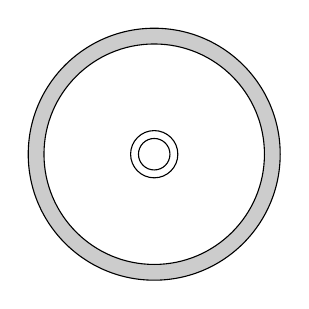
\begin{tikzpicture}
      \fill[gray!40] (2,2) circle (1.6cm);
      \fill[white] (2,2) circle (1.4cm);
      \fill[white] (2,2) circle (.2cm);
      \draw (2,2) circle (1.6cm);
      \draw (2,2) circle (1.4cm);
      \draw (2,2) circle (.2cm);
      \draw (2,2) circle (.3cm);
    \end{tikzpicture}
    \hspace{2cm}
    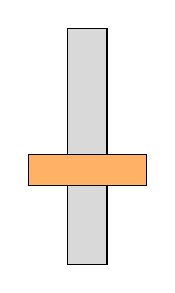
\begin{tikzpicture}
         \fill[gray!30] (0,0) rectangle (0.5,3);
         \draw (0,0) rectangle (0.5,3);
         \fill[orange!60] (-0.5,1) rectangle (1,1.4);
         \draw (-0.5,1) rectangle (1,1.4);
     \end{tikzpicture}
    \end{center}
    \begin{center}
    \end{center}
    
    \vspace{-0.5cm}
    
    % Legend
    \begin{center}
    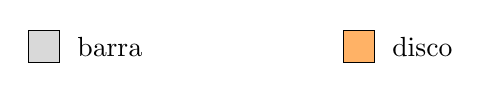
\begin{tikzpicture}
      % Gray box
      \fill[gray!30] (0,0) rectangle (0.4,0.4);
      \draw (0,0) rectangle (0.4,0.4);
      \node[anchor=west] at (0.5,0.2) {barra};
      % Orange box
      \fill[orange!60] (4,0) rectangle (4.4,0.4);
      \draw (4,0) rectangle (4.4,0.4);
      \node[anchor=west] at (4.5,0.2) {disco};
    \end{tikzpicture}
    \end{center}
\caption{Representación de la barra junto con el disco ferromagnético}
\end{figure}



\section{Movimiento asociado al efecto Stick-slip}
El contacto entre superficies genera fricción, lo que impacta en el rendimiento de tareas de alta precisión; adicionalmente, su influencia tanto estática como dinámica puede producir inestabilidad en sistemas de control de lazo cerrado. Por otro lado, tenemos que el efecto de zona muerta complejiza aún más el diseño de controladores, pero eso requiere hacer una descripción de estos fenómenos que originan la zona muerta.

Se redujo el estudio de los modelos de fricción desde los más simples como el modelo de  fricción viscosa y el modelo de fricción de Coulomb, por ser los modelos más utilizados en sistemas de control de modelos mecánicos, hasta el modelo de Stribeck, un modelo más elaborado que incorpora los modelos anteriores y que adicionalmente captura el comportamiento del movimiento a bajas velocidades.
\begin{itemize}
    \item Viscosa
    \item Coulomb
    \item Estática
    \item Stribeck
\end{itemize}





\subsection{Fricción viscosa}
La fricción viscosa es proporcional a la velocidad relativa:
\(F_{visc} = -\alpha v\)
\begin{center}
\begin{tikzpicture}
  \begin{axis}[
    axis lines = left,
    xlabel = {$v$ (m/s)},
    ylabel = {$F_{visc}$ (N)},
    width=7cm,
    height=6cm,
    legend style={at={(0.5,-0.15)}, anchor=north},
    domain=0:5,
    samples=100
  ]
    \addplot[
      color=blue,
      thick
    ] {x}; 
  \end{axis}
\end{tikzpicture}
\end{center}

\subsection{Fricción de Coulomb}
La fricción de Coulomb es proporcional al signo de la velocidad relativa:
\(F_{coul} = \beta \, \operatorname{sgn}(v)\)

\begin{center}
    \begin{tikzpicture}
    \begin{axis}[
        axis lines=middle,
        xlabel={$v$},
        ylabel={$F_{\text{coul}}$},
        xtick={-2, -1, 0, 1, 2},
        ytick={-1, 0, 1},
        ymin=-1.5, ymax=1.5,
        xmin=-2.5, xmax=2.5,
        domain=-2.5:2.5,
        samples=100,
        width=10cm, height=6cm,
        thick
    ]
    \pgfmathsetmacro{\beta}{1} 
    \addplot[blue, very thick, domain=-2.5:-0.01] {- \beta };
    \addplot[blue, very thick, domain=0.01:2.5] { 1 };
    \addplot[only marks, mark=*, mark size=2pt, fill=white, draw=blue] coordinates {(0,0)};
    \end{axis}
\end{tikzpicture}
\end{center}


\subsection{Fricción estática}
La fricción estática mantiene el cuerpo en su lugar hasta que la fuerza aplicada sobre el mismo excede algún valor \(\mu\), dependiendo de la rugosidad de las superficies.

\subsection{Fricción de Stribeck}
La fricción de Stribeck es una versión refinada de la fricción de Coulomb está se caracteriza por presentar una reducción de la fricción cuando la velocidad incrementa, pero que aún se encuentra en un rango de valores bajos.
\(F_{str} = \gamma \, \operatorname{sgn}(v)e^{-2|v|}\)

\begin{center}
 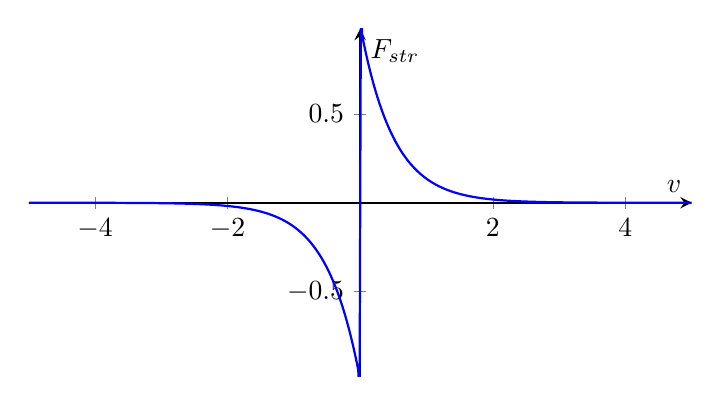
\begin{tikzpicture}
    \begin{axis}[
        axis lines=middle,
        xlabel={$v$},
        ylabel={$F_{str}$},
        width=10cm,
        height=6cm,
        domain=-5:5,
        samples=500,
        thick
    ]
    \addplot[
        blue,
        smooth
    ]
    {sign(x) * exp(-2 * abs(x))};
    \end{axis}
\end{tikzpicture}   
\end{center}




